\documentclass[12pt]{article}
\usepackage{amsmath}
\usepackage{array}
% \usepackage{gensymb}
\usepackage{geometry}
\usepackage{graphicx}
\usepackage{pgfplots}
\usepackage{siunitx}
\usepackage{wrapfig}

\title{Homework \#13}
\author{Donald Aingworth IV}
\date{November 20, 2024}

\pgfplotsset{width=8cm,compat=1.9}
\usepgfplotslibrary{external}
% \tikzexternalize

\begin{document}

\DeclareSIUnit{\mile}{mi}
\DeclareSIUnit{\gal}{gal}
\DeclareSIUnit{\foot}{ft}
\DeclareSIUnit{\h}{h}
\DeclareSIUnit{\rad}{rad}
\DeclareSIUnit{\u}{u}

\maketitle

\pagebreak

\section*{Problem 1}
\begin{wrapfigure}{r}{0.35\textwidth}
    \vspace{-30pt}
    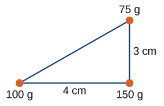
\includegraphics[width=0.35\textwidth]{graph_1.png} 
    % \label{fig:wrapfig}
\end{wrapfigure}
Three point masses are placed at the corners of a triangle as shown in the figure below. Find the
center of mass of the three-mass system.

\subsection*{Solution}
To do this, we add up the masses times their positions and divide that by the total mass.
\begin{align}
    \bar{x} &=  \frac{\sum m_i*x_i}{\sum m_i}
        =   \frac{100*0 + 75*4 + 150*4}{100 + 75 + 150}
        =   \frac{900}{325}
        =   \boxed{2.769 \unit{\centi\meter}}\\
    \bar{y} &=  \frac{\sum m_i*y_i}{\sum m_i}
        =   \frac{100*0 + 150*0 + 75*3}{100 + 75 + 150}
        =   \frac{225}{325}
        =   \boxed{0.692\unit{\centi\meter}}
\end{align}

\pagebreak
\section*{Problem 2}
Find the center of mass of a rod of length L whose mass density changes from one end to the other
quadratically. That is, if the rod is laid out along the x-axis with one end at the origin and the other end
at $x = L$, the density is given by $\rho(x) = \rho_0 + (\rho_1 - \rho_0) \left(\frac{x}{L}\right)^2$, where $\rho_0$ and $\rho_1$ are constant values.

\subsection*{Solution}


\pagebreak
\section*{Problem 3}
\begin{wrapfigure}{r}{0.35\textwidth}
    \vspace{-30pt}
    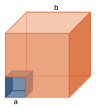
\includegraphics[width=0.35\textwidth]{graph_3.png} 
    % \label{fig:wrapfig}
\end{wrapfigure}
A cube of side a is cut out of another cube of side b as shown in the figure below. Find the location of
the center of mass of the structure. (Hint: Think of the missing part as a negative mass overlapping a
positive mass.)

\subsection*{Solution}


\pagebreak
\section*{Problem 4}
Two skaters, one with mass 65 kg and the other with mass 40 kg, stand on an ice rink holding a pole
of length 10 m and negligible mass. Starting from the ends of the pole, the skaters pull themselves along
the pole until they meet. How far does the 40 kg skater move?

\subsection*{Solution}


\pagebreak
\section*{Problem 5}
What is the average momentum of an avalanche that moves a 40-cm-thick layer of snow over an area
of 100 m by 500 m over a distance of 1 km down a hill in 5.5 s? Assume a density of 350 kg/m3 for the
snow.

\subsection*{Solution}


\pagebreak
\section*{Problem 6}
\begin{wrapfigure}{r}{0.35\textwidth}
    \vspace{-30pt}
    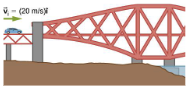
\includegraphics[width=0.35\textwidth]{graph_6.png} 
    % \label{fig:wrapfig}
\end{wrapfigure}
A 75.0-kg person is riding in a car moving at 20.0 m/s when the car runs into a bridge abutment
(see the following figure). a. Calculate the average force on the person if he is stopped by a padded
dashboard that compresses an average of 1.00 cm. Calculate the average force on the person if he is
stopped by an air bag that compresses an average of 15.0 cm.

\subsection*{Solution}


\pagebreak
\section*{Problem 7}
\begin{wrapfigure}{r}{0.35\textwidth}
    \vspace{-30pt}
    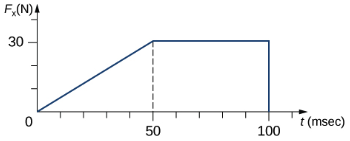
\includegraphics[width=0.35\textwidth]{graph_7.png} 
    % \label{fig:wrapfig}
\end{wrapfigure}
The x-component of a force on a 46-g golf ball by a 7-iron versus time is plotted in the following
figure. (a). Find the x-component of the impulse during the intervals i. [0, 50 ms], and ii. [50 ms, 100 ms]
(b) Find the change in the x-component of the momentum during the intervals iii. [0, 50 ms], and iv. [50
ms, 100 ms]

\subsection*{Solution}


\pagebreak
\section*{Problem 8}
\begin{wrapfigure}{r}{0.35\textwidth}
    \vspace{-30pt}
    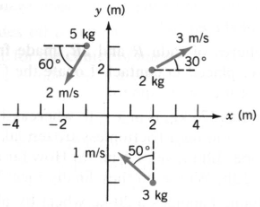
\includegraphics[width=0.35\textwidth]{graph_8.png} 
    % \label{fig:wrapfig}
\end{wrapfigure}
The instantaneous positions and velocities of three particles are shown in the figure below. Find: (a)
the position of the CM; (b) the velocity of the CM; (c) the position of the CM 3.00 s later if there is no
external force acting.

\subsection*{Solution}
\subsubsection*{Section (a)}
The position of the center of mass can be calculated by multiplying the masses by the positions and dividing by the total mass.
\begin{align}
    (\bar{x},\bar{y})   &=  \frac{\sum m_i*(x_i,y_i)}{\sum m_i}
        =   \frac{5*(-1,3) + 2*(2,2) + 3*(2,-3)}{5 + 2 + 3}\\
        &=  \frac{(-5,15) + (4,4) + (6,-9)}{10} = \frac{(5,10)}{10}
        =   \boxed{\left(\frac{1}{2}\unit{\meter},1\unit{\meter}\right)}
\end{align}

\subsubsection*{Section (b)}
The velocity of the center of mass would here be calculatable by the same process but with velocity rather than postion.
\begin{align}
    \vec{u}(\theta) &=  (\cos(\theta),\sin(\theta))\\
    \vec{v} &=  \frac{\sum m_i*v_i}{\sum m_i}
            =   \frac{5*2*\vec{u}(240\unit{\degree}) + 2*3*\vec{u}(30\unit{\degree}) + 3*1*\vec{u}(140\unit{\degree})}{5 + 2 + 3}\\
            &=  \frac{5(-1,-\sqrt{3}) + 3(\sqrt{3},1) + 3(-0.766,0.643)}{10}\\
            &=  \frac{(-5,-5\sqrt{3}) + (3\sqrt{3},3) + (-2.298, 1.928)}{10}\\
            &=  \frac{(-2.102,-3.732)}{10}
            =   \boxed{(-0.2102,-0.3732) \unit{\meter/\second}}
\end{align}

\subsubsection*{Section (c)}
We can apply the position-velocity formula now that we know the 


\end{document}